\documentclass[dvipdfmx,autodetect-engine,titlepage]{jsarticle}
\usepackage[dvipdfm]{graphicx}
\usepackage{ascmac}
\usepackage{fancybox}
\usepackage{listings}
\usepackage{plistings}
\usepackage{itembkbx}
\usepackage{amsmath}
\usepackage{svg}
\usepackage{url}
\usepackage{graphics}
\usepackage{listings,jvlisting}
\usepackage{scalefnt}

\textheight=23cm
\renewcommand{\figurename}{図}
\renewcommand{\tablename}{表}
\newenvironment{code}
{\vspace{0.5zw}\VerbatimEnvironment  
\begin{screen} 
\baselineskip=1.0\normalbaselineskip
 \begin{Verbatim}}
{\end{Verbatim}
\baselineskip=\normalbaselineskip
 \end{screen}\vspace{0.5zw}} 

 \lstset{
    basicstyle={\ttfamily},
    identifierstyle={\small},
    commentstyle={\smallitshape},
    keywordstyle={\small\bfseries},
    ndkeywordstyle={\small},
    stringstyle={\small\ttfamily},
    frame={tb},
    breaklines=true,
    columns=[l]{fullflexible},
    numbers=left,
    xrightmargin=0zw,
    xleftmargin=3zw,
    numberstyle={\scriptsize},
    stepnumber=1,
    numbersep=1zw,
    lineskip=-0.5ex
    }

\title{情報理工学部 SNコース 2回\\
セキュリティ・ネットワーク学実験2\\
課題6レポート}
\author{2600200443-6\\Yamashita Kyohei\\山下 恭平}
\date{December 21 2021}

\begin{document}

\maketitle

\section{概要}
TCPを用いて、接続許可リストにあるクライアントのみに対し、サーバが保有しているファイル一覧
を送信し、クライアントから指定されたファイルを送信するプログラムを作成する。
ネットワークセキュリティの向上を意図して、許可されたIPアドレスを持つクライアント
だけが、通信を行うように実装した。

\section{外部仕様}

\subsection{サーバ側}
サーバは起動と同時にクライアントからの接続を待機する。許可されたクラインアント
から接続が行われた時、図1のように接続先のIPアドレスを表示し、送信したファイル名
を表示し、通信を終了する。

\begin{figure}[h]
    \centering
    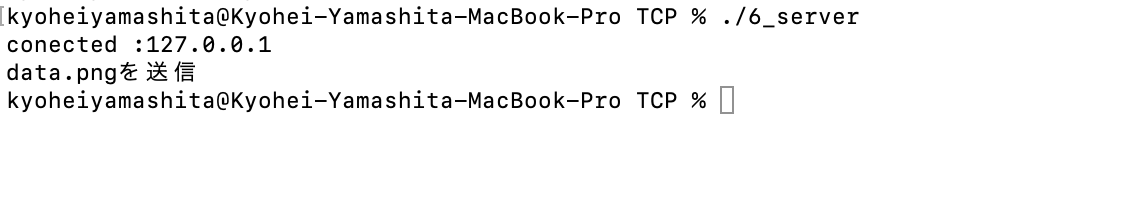
\includegraphics[scale=1]{pic3.png}
    \caption{許可した相手との通信}
\end{figure}

許可されていない相手から通信が行われた場合は図2のように、許可されていない
趣旨を表示し、通信を終了する。

\begin{figure}[h]
    \centering
    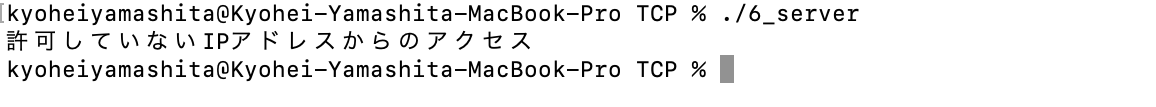
\includegraphics[scale=1]{pic5.png}
    \caption{許可していない相手との通信}
\end{figure}

\subsection{クライアント側}
クライアントは起動時、図3のように、第二引数にホスト名、第三引数にポート番号を
入力する必要がある。

\begin{figure}[h]
    \centering
    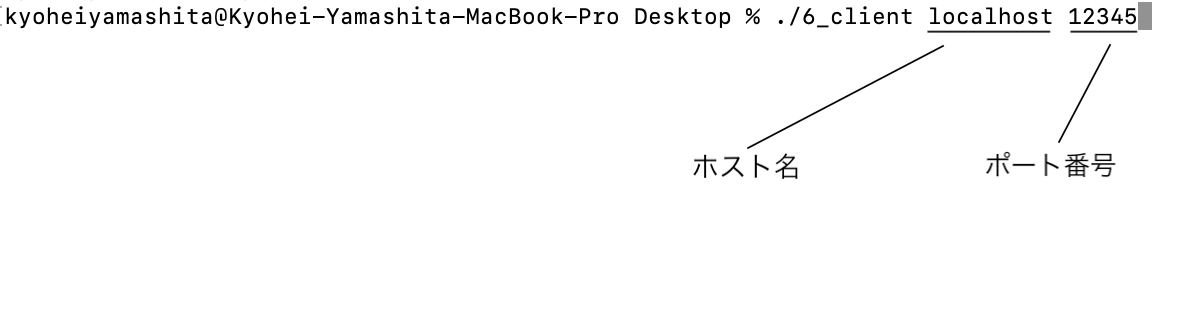
\includegraphics[scale=0.8]{pic1.png}
    \caption{クライアント起動時}
\end{figure}

指定した相手と接続を行うとき、初めに入力したホスト名のIPアドレスを表示し、
サーバにあるダウンロード可能ファイル一覧を表示する。ファイル一覧が表示された後
、ダウンロードしたいファイル番号をキーボードから入力することでダンロードを行う
ことができる。図4はダウンロードまでの様子を示したものである。

\begin{figure}[h]
    \centering
    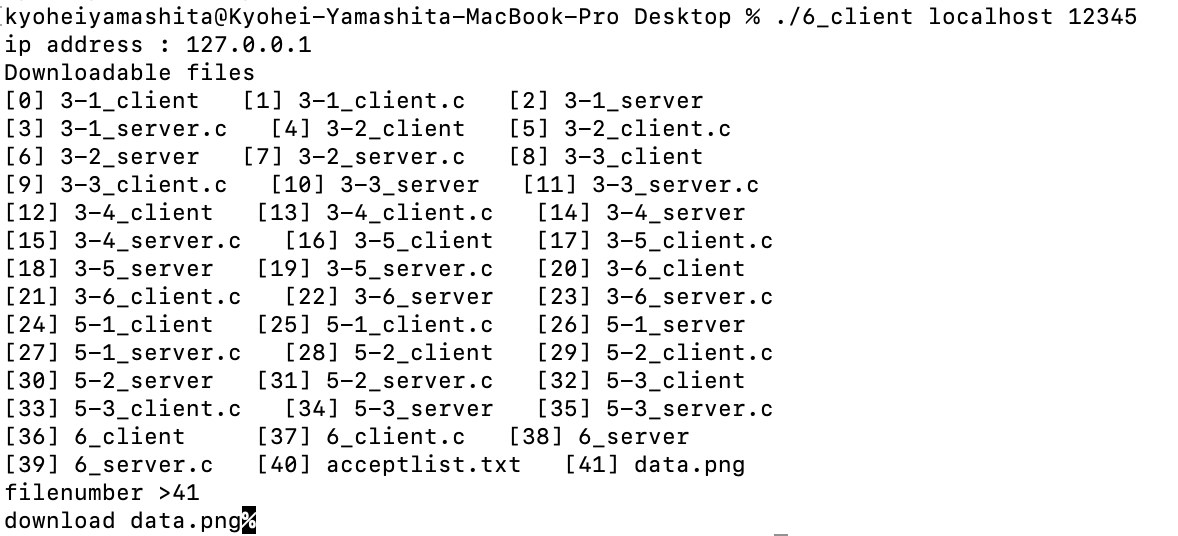
\includegraphics[scale=0.8]{pic2.png}
    \caption{サーバと通信を行う時}
\end{figure}

もし、自信のIPアドレスがサーバに許可されていない時、"connection refused"
と表示する。

\begin{figure}[h]
    \centering
    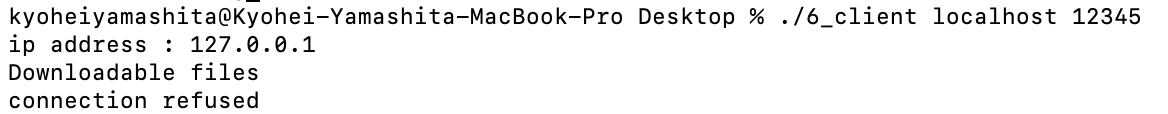
\includegraphics[scale=0.8]{pic4.png}
    \caption{IPアドレスが許可されていないとき}
\end{figure}

\section{内部使用}

\subsection{サーバ側}
サーバ側ではファイル名を取得するときにlsコマンドを使用している。lsコマンドを
仕様するにあたって、サーバがあるディレクトリを自身で設定する必要がある。この処理を
「char *cmd」に書き込むことで行っている。クライアントと接続後、「acceptlist.txt」
から許可されたIPアドレスを読み込み、クライアントのIPアドレスと比較を行い、一致
するものがない場合、クライアントに「refuse」と送り通信を終了する。IPアドレスが
許可されているとき、lsコマンドを実行し、ファイル名一覧をクライアントへ送信する。
クライアントから送り返されたファイル名のファイルを再びクライアントへ書き込むことで
、通信を終了する。

\subsection{クライアント側}
クライアント側ではサーバに接続後、サーバからファイル名一覧が送信されてくるので、
それを配列filenamesに格納する、その後、ダウンロードしたいファイルを指定しファイル名を
サーバへ送り返し、送られてきたファイルをreadすることでファイルを取得している。
もし、サーバから「refuse」の文字列が送られてきた時、IPアドレスが許可されていないので、
その趣旨を示すメッセージを出力し通信を終了する。

\section{実行例}
今回の実行では以下の内容を「acceptlist.txt」に書き込んだ。この時、自身の
IPアドレスは「192.168.11.14」である。

\begin{lstlisting}[caption = acceptlist.txt]
    192.168.11.14
    
\end{lstlisting}

今回は自分IPアドレスからの接続は許可されているので、サーバからファイル一覧が送られて
おり、指定したファイルをダウンロードすることができている。実行の様子を図6に示す。\\

\begin{figure}[h]
    \centering
    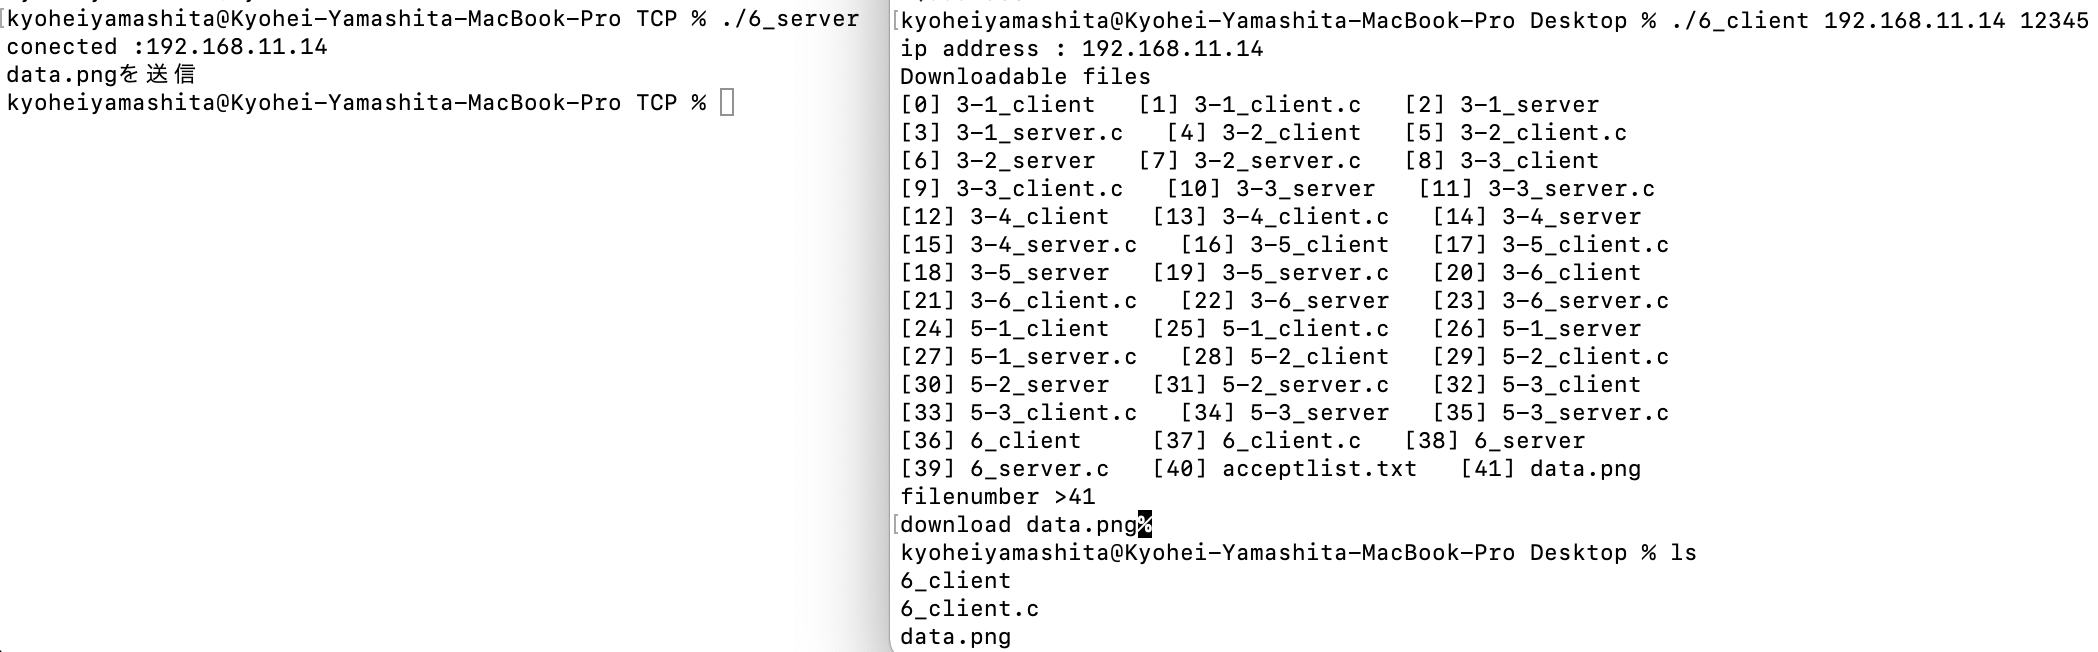
\includegraphics[scale=0.45]{pic7.png}
    \caption{IPアドレスが許可されている時}
\end{figure}

しかし、localhoat(127.0.0.1)からの接続は許可されていないので、サーバから
ファイル一覧が送られてくることはなく、警告文を表示して即座に通信を終了している。
実行の様子を図7に示す。\\

\begin{figure}[h]
    \centering
    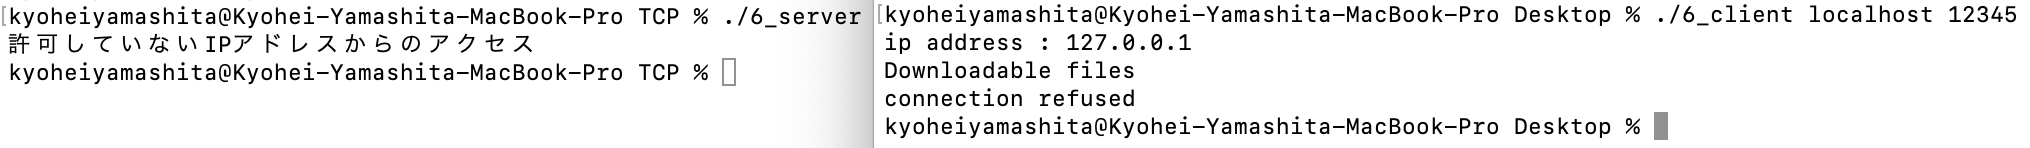
\includegraphics[scale=0.5]{pic6.png}
    \caption{IPアドレスが許可されていないとき}
\end{figure}

\section{ソースコード}
以下はソースコードである、コードの説明はコード内のコメントアウトにて行っている。
\subsection{サーバ側}

\begin{lstlisting}[caption=server,label=server.c]
#include <stdio.h>
#include <unistd.h>
#include <stdlib.h>
#include <sys/types.h>
#include <sys/socket.h>
#include <netinet/in.h>
#include <arpa/inet.h>
#include <pthread.h>
#include <errno.h>
#include <string.h>
#include <fcntl.h>

//fgets()の改行文字を削除するための関数
void lntrim(char *str)
{
    char *p;
    p = strchr(str, '\n');
    if (p != NULL)
    {
        *p = '\0';
    }
}

int main(int argc, char *argv[])
{
    int sock0;
    struct sockaddr_in addr;
    struct sockaddr_in client;
    socklen_t len;
    int sock;
    int errocheck;
    int fd,ret,n;
    char buf[2048];
    char str[256];

    //サーバがあるディレクトリのパスを入力
    char *cmd = "/bin/ls /Users/kyoheiyamashita/VSCode/NW実験/TCP";

    //許可するIPアドレス一覧表
    char fname[] = "acceptlist.txt";

    FILE *fp; // FILE型構造体
    int refusecheck = 0;

    /* ソケットの作成 */
    sock0 = socket(AF_INET, SOCK_STREAM, 0);
    if (sock0 < 0)
    {
        perror("socket");
        printf("%d\n", errno);
        return 1;
    }

    /* ソケットの設定 */
    addr.sin_family = AF_INET;
    addr.sin_port = htons(12345);
    addr.sin_addr.s_addr = INADDR_ANY;
    errocheck = bind(sock0, (struct sockaddr *)&addr, sizeof(addr));
    if (errocheck < 0)
    {
        perror("bind");
        printf("%d\n", errno);
        return 1;
    }

    /* TCPクライアントからの接続要求を待てる状態にする */
    errocheck = listen(sock0, 5);
    if (errocheck < 0)
    {
        perror("listen");
        printf("%d\n", errno);
        return 1;
    }

    /* TCPクライアントからの接続要求を受け付ける */
    len = sizeof(client);

    sock = accept(sock0, (struct sockaddr *)&client, &len);
    if (sock < 0)
    {
        perror("accept");
        printf("%d\n", errno);
        return 1;
    }

    fp = fopen(fname, "r"); // ファイルを開く。失敗するとNULLを返す。
    if (fp == NULL)
    {
        printf("%s file not open!\n", fname);
        return -1;
    }

    //テキストファイルからIPアドレスを読み込み//
    while (fgets(str, 256, fp) != NULL)
    {
        int l = 0;

        while (1)
        {
            if (str[l] == '\n')
            {
                str[l] = '\0';
                break;
            }

            l++;
        }

        //テキスト内に一致するIPアドレスがあればそのIPアドレスを表示//
        if (strcmp(str, inet_ntoa(client.sin_addr)) == 0)
        {
            printf("conected :%s\n", str);

            refusecheck = 1;

            fclose(fp);

            break;
        }
    }

    //一致するIPアドレスがない時//
    if (refusecheck == 0)
    {
        puts("許可していないIPアドレスからのアクセス");

        strcpy(buf,"refuse");

        //クライアントへ「refuse」と送信//
        write(sock, buf, sizeof(buf));

        //通信の終了//
        close(sock);
        close(sock0);
        return 0;
    }

    //lsコマンドでディレクトリ内のファイル名を取得//
    if ((fp = popen(cmd, "r")) != NULL)
    {
        while (fgets(buf, sizeof(buf), fp) != NULL)
        {
            lntrim(buf);

            //ファイル名をクライアントへ送信
            write(sock, buf, sizeof(buf));
        }

        pclose(fp);
    }

    //クライアント側readを止めるための文字列を送信//
    errocheck = write(sock, "HELLO", 5);
    if (errocheck < 0)
    {
        perror("write");
        printf("%d\n", errno);
        return 1;
    }

    //クライアントから送信するファイル名を受信//
    read(sock, buf, sizeof(buf));

    printf("%sを送信\n",buf);

    //指定されたファイルをオープン//
    fd = open(buf, O_RDONLY);
    if (fd < 0)
    {
        close(sock);

        close(sock0);

        return 0;
    }

    //ファイルをクライアントへ送信//
    while ((n = read(fd, buf, sizeof(buf))) > 0)
    {
        ret = write(sock, buf, n);
        if (ret < 1)
        {
            perror("write");
            break;
        }
    }

    /* TCPセッションの終了 */
    close(sock);

    /* listen するsocketの終了 */
    close(sock0);

    return 0;
}


\end{lstlisting}

\subsection{クライアント側}

\begin{lstlisting}[caption=client,label=client.c]
#include <stdio.h>
#include <stdlib.h>
#include <string.h>
#include <unistd.h>
#include <sys/types.h>
#include <sys/socket.h>
#include <netinet/in.h>
#include <arpa/inet.h>
#include <errno.h>
#include <netdb.h>
#include <errno.h>
#include <fcntl.h>

int main(int argc, char *argv[])
{
    struct sockaddr_in server;
    struct addrinfo hints, *res;
    struct in_addr addr;
    int sock;
    char buf[2048];
    char filenames[1024][2048];
    int n;
    int errocheck;
    int portnum;
    int fd;
    int filecount = 0;
    int filenumber;
    char ipadd[16];

    //ホスト名をIPアドレスへ変換
    portnum = atoi(argv[2]);

    memset(&hints, 0, sizeof(hints));
    hints.ai_socktype = SOCK_STREAM;
    hints.ai_family = AF_INET;
    if ((errocheck = getaddrinfo(argv[1], NULL, &hints, &res)) != 0)
    {
        printf("error %d\n", errocheck);
        return 1;
    }

    addr.s_addr = ((struct sockaddr_in *)(res->ai_addr))->sin_addr.s_addr;
    inet_ntop(AF_INET, &addr, ipadd, sizeof(ipadd));
    printf("ip address : %s\n", ipadd);

    /* ソケットの作成 */
    sock = socket(AF_INET, SOCK_STREAM, 0);
    if (sock < 0)
    {
        perror("socket");
        printf("%d\n", errno);
        return 1;
    }

    /* 接続先指定用構造体の準備 */
    server.sin_family = AF_INET;
    server.sin_port = htons(portnum);

    /* 127.0.0.1はlocalhost */
    inet_pton(AF_INET, ipadd, &server.sin_addr.s_addr);

    /* サーバに接続 */
    errocheck = connect(sock, (struct sockaddr *)&server, sizeof(server));
    if (errocheck < 0)
    {
        perror("connect");
        printf("%d\n", errno);
        return 1;
    }

    memset(buf, 0, sizeof(buf));

    puts("Downloadable files");

    //"HELLO"が送られてくるまでサーバからファイル名を受信する
    while ((n = read(sock, buf, sizeof(buf))) > 0)
    {

        if (strcmp(buf, "HELLO") == 0)
        {
            break;
        }

        //IPアドレスが許可されていない場合"refuzed"が送られてくる。
        if (strcmp(buf, "refuse") == 0)
        {
            puts("connection refused");

            close(sock);

            return 0;
        }

        printf("[%d] %-10s   ", filecount, buf);

        //受信したファイル名を配列へ格納
        strcpy(filenames[filecount], buf);

        filecount++;

        if ((filecount % 3) == 0)
        {
            putchar('\n');
        }

        memset(buf, 0, sizeof(buf));
    }

    //受信したいファイルを選択//
    printf("filenumber >");

    scanf("%d", &filenumber);

    printf("download %s", filenames[filenumber]);

    //受信したいファイル名をサーバへ送信//
    write(sock, filenames[filenumber], sizeof(filenames[filenumber]));

    //ファイル書き込み用の空のファイルを生成//
    fd = open(filenames[filenumber], O_WRONLY | O_CREAT | O_EXCL, 0600);
    if (fd < 0)
    {
        puts("すでに同じ名前のファイルが存在");

        write(sock, "erro", sizeof("erro"));

        close(sock);

        return 1;
    }

    //サーバから送られてきたデータの読み込みと書き込み//
    while ((n = read(sock, buf, sizeof(buf))) > 0)
    {
        errocheck = write(fd, buf, n);

        if (errocheck < 1)
        {
            perror("write");
            break;
        }
    }

    /* socketの終了 */
    close(sock);

    return 0;
}


\end{lstlisting}


\end{document}

